\begin{figure*}[t]
    \centering
    \subcaptionbox{BM as a particular case of OT with no regularization ($\epsilon = 0$). The \emph{Hungarian algorithm} obtains the same solution.%
        \label{fig:params-influence-bipartite}}[.45\textwidth]%
        {\def\svgwidth{0.35\textwidth}\footnotesize
        	\graphicspath{{chapters/uotod/image/matchings/}}
        	\import{chapters/uotod/image}{matchings/G1.pdf_tex} }%
    \hfill%
    \subcaptionbox{OT with regularization ($\epsilon \neq 0$). The regularization smoothens the matching allowing for multiple connections.The problem here is fully balanced ($\tau_1, \tau_2 \rightarrow \infty$).
        \label{fig:params-influence-reg}}[.45\textwidth]%
        {\def\svgwidth{0.35\textwidth}\footnotesize
        	\graphicspath{{chapters/uotod/image/matchings/}}
        	\import{chapters/uotod/image}{matchings/G2.pdf_tex} }%
    \hfill%
    \subcaptionbox{Unbalanced OT with regularization ($\epsilon \neq 0$ and $\tau_1 \ll \tau_2$). The smoothing is also visible.%
        \label{fig:params-influence-unbalanced}}[.45\textwidth]%
        {\def\svgwidth{0.35\textwidth}\footnotesize
        	\graphicspath{{chapters/uotod/image/matchings/}}
        	\import{chapters/uotod/image}{matchings/G3.pdf_tex} }%
    \hfill%
    \subcaptionbox{Matching each ground truth object to the closest prediction as Unbalanced OT without regularization with $\epsilon=0$, $\tau_1 = 0$ and $\tau_2 \rightarrow \infty$.%
        \label{fig:params-influence-min}}[.45\textwidth]%
        {\def\svgwidth{0.35\textwidth}\footnotesize
        	\graphicspath{{chapters/uotod/image/matchings/}}
        	\import{chapters/uotod/image}{matchings/G4.pdf_tex} }%
    \caption{Example of the influence of the parameters. The blue dots represent predictions $\hat{\mathbfit{y}}_i$. The red squares represent ground truth objects $\mathbfit{y}_j$. The distributions $\mathbfit{\alpha}$ and $\mathbfit{\beta}$ are defined as in Prop.~\ref{prop:lap}. The thickness of the lines is proportional to the amount transported $P_{i,j}$. Only sufficiently thick lines are plotted. The dummy \emph{background} ground truth $\mathbfit{y}_{N_g+1} = \varnothing$ is not shown, nor are the connections to it. We can see that the plots~\subref{fig:params-influence-bipartite} and~\subref{fig:params-influence-reg} are balanced and the mass constraints are respected ($\mathbfit{P} \in \mathcal{U}(\mathbfit{\alpha},\mathbfit{\beta})$). This can be seen graphically by noticing that the thickness of the lines sum up to the same mass for each red point.}
    \label{fig:params-influence}
\end{figure*}

\section{Optimal Transport}
In this section, we show how \emph{Optimal Transport} and then its \emph{Unbalanced} extension unify both the \emph{Hungarian algorithm} used in DETR~\cite{carion2020detr}, and matching each prediction to the closest ground truth object used in both Faster R-CNN~\cite{ren2015fasterrcnn} and SSD~\cite{liu2016ssd}. We furthermore stress the advantages of entropic regularization, both computationally and qualitatively. This allows us to explore a new continuum of matching methods, with varying properties.

\begin{definition}[Optimal Transport]
\label{def:OT}
    Given a distribution $\mathbfit{\alpha} \in \Delta^{N_p}$ associated to the predictions $\{\hat{\mathbfit{y}}_i\}_{i=1}^{N_p}$, and another distribution $\mathbfit{\beta} \in \Delta^{N_g}$ associated with the ground truth  objects $\{\mathbfit{y}_j\}_{j=1}^{N_g}$. Let us consider a pair-wise matching cost $\mathcal{L}_{\text{match}}(\hat{\mathbfit{y}}_i,\mathbfit{y}_j)$ between a prediction $\hat{\mathbfit{y}}_i$ and a ground truth object $\mathbfit{y}_j$. We now define \emph{Optimal Transport (OT)} as finding the match $\mathbfit{P}$ that minimizes the following problem:
    \begin{equation}
        \hat{\mathbfit{P}} = \underset{\mathbfit{P} \,\in\, \mathcal{U}(\mathbfit{\alpha},\mathbfit{\beta})}{\mathrm{arg\,min}} \left\{\sum_{i,j=1}^{N_p,N_g} P_{i,j}\mathcal{L}_{\text{match}}\left(\hat{\mathbfit{y}}_i, \mathbfit{y}_j \right)\right\},
    \end{equation}
    with transport polytope ( the set of all admissible solutions) 
    \begin{equation}
        \mathcal{U}(\mathbfit{\alpha},\mathbfit{\beta}) = \left\{ \mathbfit{P} \in \mathbb{R}_{\geq 0}^{N_p \times N_g} : \sum_{j=1}^{N_g} P_{i,j} = \alpha_i ,\sum_{i=1}^{N_p} P_{i,j} = \beta_j\right\}.
    \end{equation}
\end{definition}
Provided that certain conditions apply to the underlying cost $\mathcal{L}_{\text{match}}$, the minimum defines a distance between $\mathbfit{\alpha}$ and $\mathbfit{\beta}$, referred to as the Wasserstein distance $\mathcal{W}(\mathbfit{\alpha},\mathbfit{\beta})$ (for more information, we refer to monographs~\cite{villani2009optimal,santambrogio,peyre2019computational}; see also Appendix~\ref{app:theory-wass}).

\subsection{The Hungarian Algorithm}
The Hungarian algorithm solves the \emph{Bipartite Matching} (BM). We will now show how this is a particular case of Optimal Transport.
%\footnote{When unclear from the context, it may be fully referred to as \emph{Minimum Cost Bipartite Matching}. Alternate denominations are also encountered, such as the \emph{Linear Assignment Problem},  \emph{Minimal Assignment Problem} or \emph{Hungarian matching}, referring to one of the algorithms solving the problem. Sometimes the malapropism \emph{Hungarian algorithm} also may refer to it rather than the procedure to solve it.}. 

% \subsubsection{Bipartite Matching}
\begin{definition}[Bipartite Matching]
\label{def:lap}
Given the same objects as  in Definition~~\ref{def:OT}, the \emph{Bipartite Matching (BM)} minimizes the cost of the pairwise matches between the ground truth objects with the predictions:
\begin{equation}
    \hat{\sigma} = \mathrm{arg\, min} \left\{\sum_{j=1}^{N_g} \mathcal{L}_{\text{match}}\left(\hat{\mathbfit{y}}_{\sigma(j)},  \mathbfit{y}_{j} \right): \sigma \in \mathcal{P}_{N_g}(\llbracket N_p \rrbracket)\right\},
\end{equation}
where $\mathcal{P}_{N_g}(\llbracket N_p\rrbracket) = \left.\big\{\sigma \in \mathcal{P}(\llbracket N_p \rrbracket) \,\right| |\sigma| = N_g \big\}$ is the set of possible combinations of $N_g$ in $N_p$, with $\mathcal{P}(\llbracket N_p \rrbracket)$ the power set of $\llbracket N_p\rrbracket$ (the set of all subsets).
\end{definition}
%
BM tries to assign each ground truth $\mathbfit{y}_j$ to a different prediction $\hat{\mathbfit{y}}_i$ in a way to minimize the total cost. In contrast to OT, BM does not consider any underlying distributions $\mathbfit{\alpha}$ and $\mathbfit{\beta}$, all ground truth objects and predictions are implicitly considered to be of same mass. Furthermore, it only allows one ground truth to be matched to a unique prediction, some of these predictions being left aside and matched to nothing (which is then treated as a matching to the background $\varnothing$). The OT must match all ground truth objects to all predictions, not allowing any predictions to be left aside. However, the masses of the ground truth objects are allowed to be split between different predictions and inversely, as long as their masses correctly sum up ($\mathbfit{P} \in \mathcal{U}(\mathbfit{\alpha},\mathbfit{\beta})$).

\subsubsection{Particular Case of OT}
A solution for an imbalanced number of predictions compared to the number of ground truth objects would be to add dummy ground truth objects---the background $\varnothing$---to even the balance. Concretely, one could add a new ground truth $\mathbfit{y}_{N_g+1} = \varnothing$, with the mass equal to the unmatched number of predictions. In fact, doing so directly results in performing a BM.

\begin{proposition}
\label{prop:lap}
    The Hungarian algorithm with $N_p$ predictions and $N_g \leq N_p$ ground truth objects is a particular case of OT with $\mathbfit{P} \in \mathcal{U}(\mathbfit{\alpha},\mathbfit{\beta}) \subset \mathbb{R}^{N_p \times (N_g+1)}$, consisting of the predictions and the ground truth objects, with the background added $\{\mathbfit{y}_j\}_{j=1}^{N_g+1} = \{\mathbfit{y}_j\}_{j=1}^{N_g} \cup \big(\mathbfit{y}_{N_g+1}=\varnothing\big)$. The chosen underlying distributions are
    \begin{eqnarray}
        \mathbfit{\alpha} &=& \frac{1}{N_p}[\; \underbrace{1, \; 1, \;1,\; \ldots, \; 1}_{\text{$N_p$ predictions}}\;], \\
        \mathbfit{\beta} &=& \frac{1}{N_p}[\; \underbrace{1, \; 1, \; \ldots, \; 1}_{\text{$N_g$ ground truth objects}}, \; \underbrace{(N_p-N_g)}_{\text{background }\varnothing} \;],
    \end{eqnarray}
    provided the background cost is constant:
    $\mathcal{L}_{\text{match}}\left(\hat{\mathbfit{y}}_i,\varnothing\right) = c_{\varnothing}$. In particular for $j \in \llbracket N_g\rrbracket$, we have $\hat{\sigma}(j) = \left\{ i : P_{i,j} \neq 0 \right\}$, or equivalently $\hat{\sigma}(j) = \left\{ i : P_{i,j} = 1/N_p \right\}$.
\end{proposition}
\begin{proof}
    We refer to Appendix~\ref{app:proof-hungarian}.
\end{proof}

In other words, we can read the matching to each ground truth in the columns of $\hat{\mathbfit{P}}$. The last columns represents all the predictions matched to the background $\hat{\sigma}(N_g+1)$. Alternatively and equivalently, we can read the matching of each prediction $i$ in the rows, the ones being matched to the background have a $\hat{P}_{i,N_g+1} = 1/N_p$.

\subsubsection{Solving the Problem}
\label{computational}
Both OT and BM are linear programs. Using generic formulations would lead to a $\left(N_p+N_g+1\right) \times N_p\left(N_g+1\right)$ equality constraint matrix. It is thus better to exploit the particular bipartite structure of the problem. In particular, two families of algorithms have emerged: \emph{Dual Ascent Methods} and \emph{Auction Algorithms}~\cite{peyre2019computational}. The Hungarian algorithm is a particular case of the former and classically runs with an $\mathcal{O}\left(N_p^4\right)$ complexity~\cite{munkres1957algorithmstransportationhungarian}, further reduced to cubic by~\cite{hungarian-cubic}. Although multiple GPU implementations of a BM solver have been proposed~\cite{gpu-bipartite,gpu-hungarian,gpu-matching}, the problem remains poorly parallelizable because of its sequential nature. To allow for efficient parallelization, we must consider a slightly amended problem.

\subsection{Regularization}
We show here how we can replace the \emph{Hungarian algorithm} by a class of algorithms well-suited for parallelization, obtained by adding an entropy regularization.
\begin{definition}[OT with regularization]
\label{def:rOT}
    We consider a regularization parameter $\epsilon \in \mathbb{R}_{\geq 0}$. Extending Definition~\ref{def:OT} (OT), we define the \emph{Optimal Transport with regularization} as the following minimization problem:
    \begin{equation}
        \hat{\mathbfit{P}} = \underset{\mathbfit{P}\, \in\, \mathcal{U}(\mathbfit{\alpha},\mathbfit{\beta})}{\mathrm{arg\,min}} \left\{\sum_{i,j=1}^{N_p,N_g} P_{i,j}\mathcal{L}_{\text{match}}\left(\hat{\mathbfit{y}}_i, \mathbfit{y}_j\right) - \epsilon \,\mathrm{H}(\mathbfit{P}) \right\},
    \end{equation}
    with  $\mathrm{H}: \Delta^{N \times M} \rightarrow \mathbb{R}_{\geq 0} : \mathbfit{P} \mapsto -\sum_{i,j} P_{i,j}(\log(P_{i,j})-1)$ the entropy of the match $\mathbfit{P}$, with $0 \ln(0) = 0$ by definition.
\end{definition}

\begin{figure}[ht]
\vspace{-2.5em}
    \centering \footnotesize
    %{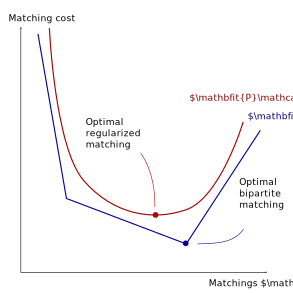
\includegraphics[width=.9\textwidth]{chapters/uotod/image/plot2.pdf_tex}}
    \import{chapters/uotod/image}{plot2.pdf_tex}
    \vspace{-.7em}
    \caption{\label{fig:ot-reg}Effect of the regularization on the minimization of the matching cost. The red line corresponds to the regularized problem ($\epsilon \neq 0$) and the blue to the unregularized one ($\epsilon = 0$).}% The machine precision curve is loosely inspired by~\cite{cuturi2013sinkhorn}.}
\end{figure}

\subsubsection{Sinkhorn's Algorithm}
The entropic regularization used when finding the match $\hat{\mathbfit{P}}$ ensures that the problem is smooth for $\epsilon \neq 0$ (see Figure~\ref{fig:ot-reg}). The advantage is that it can now be solved very efficiently using \emph{scaling algorithms} and in this particular case the algorithm of \emph{Sinkhorn}. It is particularly suited for parallelization~\cite{cuturi2013sinkhorn}, with some later speed refinements~\cite{greenkorn, screenkorn}. Reducing the regularization progressively renders the scaling algorithms numerically unstable, although some approaches have been proposed to reduce the regularization further by working in log-space~\cite{schmitzer2019stabilized,chizat2018scaling}. In the limit of $\epsilon \rightarrow 0$, we recover the exact OT (Definition~\ref{def:OT}) and the scaling algorithms cannot be used anymore. Parallelization is lost and we must resolve to use the sequential algorithms developed in Section~\ref{computational}. In brief, regularization allows to exploit GPU architectures efficiently, whereas the Hungarian algorithm and similar cannot.

\subsubsection{Smoother Matches}
When no regularization is used as in the Hungarian algorithm, close predictions and ground truth objects can exchange their matches from one epoch to the other, during the training. This causes a slow convergence of DETR in the early stages of the training~\cite{li2022dndetr}. The advantage of the regularization not only lies in the existence of efficient algorithms but also allows for a reduction of sparsity. This results in a less drastic match than the Hungarian algorithm obtains. A single ground truth could be matched to multiple predictions and inversely. The proportion of these multiple matches is controlled by the regularization parameter $\epsilon$. An illustration can be found in Figures~\ref{fig:params-influence-bipartite} and \ref{fig:params-influence-reg}.

\subsection{Unbalanced Optimal Transport}
We will now show how considering soft constraints instead of hard leads to an even greater generalization of the various matching techniques used in object detection models. In particular, matching each prediction to the closest ground truth is a limit case of the \emph{Unbalanced OT}.
\begin{definition}[Unbalanced OT]
\label{def:ruOT}
We consider two constraint parameters $\tau_1, \tau_2 \in \mathbb{R}_{\geq 0}$. Extending Definition~\ref{def:rOT} (OT with regularization), we define the \emph{Unbalanced OT with regularization}~\cite{chizat2018scaling} as the following minimization problem:
\begin{equation}
\begin{aligned}
    \hat{\mathbfit{P}} = \underset{\mathbfit{P} \in \mathbb{R}_{\geq 0}^{N_p\times N_g}}{\mathrm{arg\, min}}\biggl\{\epsilon\,\kl{\mathbfit{P}}{\mathbfit{K}_{\epsilon}}\, + & \, \tau_1\kl{\mathbfit{P}\mathbfit{1}_{N_g}}{\mathbfit{\alpha}} \\
    + & \, \tau_2\kl{\mathbfit{1}_{N_p}^\top \mathbfit{P}}{ \mathbfit{\beta}}\biggr\},
\end{aligned}%
% \begin{aligned}
%     \hat{\mathbfit{P}} = \underset{\mathbfit{P} \in \mathbb{R}_{\geq 0}^{N_p\times N_g}}{\mathrm{arg\, min}}\biggl\{\sum_{i,j=1}^{N_p,N_g} \mathcal{L}_{\text{matching}}\left(\hat{\mathbfit{y}}_i, \mathbfit{y}_j \right)P_{i,j} - \epsilon\, \mathrm{H}(\mathbfit{P})  \\
%      \qquad \qquad + \;\tau_1\kl{\mathbfit{P}\mathbfit{1}_M}{\mathbfit{\alpha}} + \tau_2\kl{\mathbfit{1}_N^\top \mathbfit{P}}{ \mathbfit{\beta}}\biggr\},
% \end{aligned}
\end{equation}
where $\mathrm{KL}: \mathbb{R}^{N\times M}_{\geq 0} \times \mathbb{R}^{N\times M}_{> 0} \rightarrow \mathbb{R}_{\geq 0}^{\phantom{N}} : (\mathbfit{U},\mathbfit{V}) \mapsto \sum_{i,j=1}^{N \times M} U_{i,j} \log(U_{i,j} / V_{i,j}) - U_{i,j} + V_{i,j}$ is the \emph{Kullback-Leibler divergence} -- also called \emph{relative entropy} -- between matrices or vectors when $M=1$, with $0 \ln (0) = 0$ by definition. The Gibbs kernel $\mathbfit{K}_{\epsilon}$ is given by $\left(K_{\epsilon}\right)_{i,j} = \exp\left(- \mathcal{L}_{\text{match}}\left(\hat{\mathbfit{y}}_i, \mathbfit{y}_j \right)/ \epsilon \right)$.
\end{definition}

We can see by development that the first term corresponds to the matching term $\mathbfit{P}\mathcal{L}_{\text{match}}$ and an extension of the entropic regularization term $\mathrm{H}(\mathbfit{P})$. The two additional terms replace the transport polytope's hard constraints $\mathcal{U}(\mathbfit{\alpha},\mathbfit{\beta})$ that required an exact equality of mass for both marginals. These new soft constraints allow for a more subtle sensitivity to the mass constraints as it allows to slightly diverge from them. It is clear that in the limit of $\tau_1, \tau_2 \rightarrow +\infty$, we recover the ``balanced'' problem (Definition~\ref{def:rOT}). This definition naturally also defines Unbalanced OT without regularization if $\epsilon = 0$. The matching term would remain and the entropic one disappear.

\subsubsection{Matching to the Closest} Another limit case is however particularly interesting in the quest for a unifying framework of the matching strategies. If the mass constraint is to be perfectly respected for the predictions ($\tau_1 \rightarrow \infty$), but not at all for the ground truth objects ($\tau_2 = 0$), it suffices to assign the closest ground truth to each prediction. The same ground truth object could be assigned to multiple predictions and another could not be matched at all, not respecting the hard constraint for the ground truth $\mathbfit{\beta}$. Each prediction however is exactly assigned once, perfectly respecting the mass constraint for the predictions $\mathbfit{\alpha}$. By assigning a low enough value to the background, a prediction would be assigned to it provided all the other ground truth objects are further. In other words, the background cost would play the role of a \emph{threshold} value.

\begin{proposition}[Matching to the closest]
\label{prop:threshold}
We consider the same objects as Proposition~\ref{prop:lap}. In the limit of $\tau_1 \rightarrow \infty$ and $\tau_2 = 0$, Unbalanced OT (Definition~\ref{def:ruOT}) without regularization ($\epsilon = 0$) admits as solution each prediction being matched to the closest ground truth object unless that distance is greater than a threshold value $\mathcal{L}_{\text{match}}\left(\hat{\mathbfit{y}}_i,\mathbfit{y}_{N_g+1}=\varnothing\right) = c_{\varnothing}$. It is then matched to the background $\varnothing$. In particular, we have
\begin{equation}
    \hat{P}_{i,j} = \left\{
    \begin{array}{ll}
        \frac{1}{N_p} & \text{if } j = \mathrm{\arg\, min}_{j \in \llbracket N_g+1 \rrbracket}\left\{\mathcal{L}_{\text{match}}\left(\hat{\mathbfit{y}}_i, \mathbfit{y}_j \right)\right\},\\
        0 & \text{otherwise}.
    \end{array}\right.
\end{equation}
\end{proposition}
\begin{proof}
    We refer to Appendix~\ref{app:proof-minimum}.
\end{proof}

\begin{figure}[h]
    \centering \footnotesize
    \import{chapters/uotod/image}{plot3.pdf_tex}
    \vspace{-.5em}
    \caption{\label{fig:unbalanced-limits}Limit cases of Unbalanced OT without regularization ($\epsilon=0$).}
\end{figure}


The converse also holds. If the ground truth objects mass constraints were to be perfectly respected ($\tau_2 \rightarrow \infty$), but not the predictions ($\tau_1 \rightarrow 0$), each ground truth would then be matched to the closest prediction. The background would be matched to the remaining predictions. Some predictions could not be matched and other ones multiple times. The limits of Unbalanced OT are illustrated in Fig.~\ref{fig:unbalanced-limits}. By setting the threshold sufficiently high, we get an exact minimum, i.e., where every prediction is matched to the closest ground truth. This can be observed in Figure~\ref{fig:params-influence-min}.

\subsubsection{Scaling Algorithm}
Similarly as before, adding entropic regularization ($\epsilon \neq 0$) to the \emph{Unbalanced OT} allows it to be solved efficiently on GPU with a scaling algorithm, as an extension of Sinkhorn's algorithm~\cite{chizat2018scaling, chizat-these}. The regularization still also allows for smoother matches, as shown in Figure~\ref{fig:params-influence-unbalanced}.


\subsubsection{Softmax}
In the limit of $\tau_1 \rightarrow +\infty$ and $\tau_2 = 0$, the solution corresponds to a softmax over the ground truth objects for each prediction. The regularization $\varepsilon$ controls then the ``softness'' of the softmax, with $\varepsilon = 1$ corresponding to the conventional softmax and $\varepsilon \rightarrow 0$ the matching to the closest. We refer to Appendix~\ref{app:softmax} for more information.

